\documentclass[titlepage]{article}
\usepackage[T1]{fontenc}
\usepackage[utf8x]{inputenc}
\usepackage[english]{babel}
\usepackage{graphicx}
\usepackage{graphicx}
\usepackage{grffile}
\usepackage{float}
\usepackage{placeins}
\usepackage{longtable}
\usepackage[dvipsnames]{xcolor}
\usepackage{listings}
\usepackage{alloy-style}
\usepackage{blindtext, rotating}
\usepackage{hyperref}
\pdfcompresslevel0


\author{Luca Massini \and Daniele Nicolò}

\title{Requirement analysis and specification document
\\  Safestreets}

\date{10 November 2019}
\begin{document}
\maketitle
\newpage 
\tableofcontents
\newpage

\section{Introduction}
The purpose of this document is to represent the Requirement Analysis and Specification Document (RASD).
This document shows what are the goals and the requirements of the software.
It has to represent how the application can be useful for the users and why they are fundamental to improve the quality of the service offered. Secondly, this document can be also used as a support for the testing of the system, for the verification activities and also the validation ones. The RASD can be also used to guide the changes in a already existing system.



\subsection{Purpose}

\subsubsection{Description of the given problem}
SafeStreets is a mobile application useful to help people to be safer when they are on the street.\\
The users can send to the municipality pictures of violations occurring in public streets: the reporting can concern violation on the road, in a parking lot and so on.\\
The software allows the users to send detailed information about the violation, such as the hour, the date, the type of violation and the position (they can be captured with GPS).\\
Furthermore, the service can provide to the user information about the streets around which he/she is,
such as the number of violations per street and consequently the level of danger of the street.\\
In addition, the user can have a different service based on the category to which he/she belongs.\\
The user and the municipality can also find on the application the most "dangerous" vehicles, that are the ones with the highest number of reports from the users.\\
The service must be different in base of the type of user, such as municipalities, motorists, motorcyclists, bikers, pedestrians, disabled people etc.\\
Finally, the users must be able to receive recommendations from the system to avoid using streets, parking lots that are risky in general or at a specific hour or date.\\
The authorities will be informed of the violations through the municipality.

\subsubsection{Goals}
\begin{itemize}
\item $[goal 1]$:  The service allows the users to report a violation to the municipality.
\begin{itemize}

	\item $[goal 1.1]$: The user must send a picture of the 			violation.
	
	\item $[goal 1.2]$: The user can specify the date and the 						hour when the violation has happened 							and the type of violation.
	

	\item $[goal 1.3]$: The municipality must be able to     	receive the reports.  \\
	
\end{itemize}

\item $[goal 2]$: The service allows the users to have detailed information about the violations and the streets safety.
      \begin{itemize}
      	\item $[goal 2.1]$: The users can know which are the 			most reported streets, areas or parking lots.
		
		\item $[goal 2.2]$: The user, in base of his/her 				position, can be recommended to use the safest 					streets/areas, etc or avoid the dangerous ones.\\

      \end{itemize}

\item $[goal 3]$: Safestreets must send to the municipality suggestions to improve the safety of the streets if and only if the municipality asks for them.
	\begin{itemize}
	\item $[goal 3.1]$: Every time the municipality makes a request in order to obtain suggestions, they must receive them by Safestreets.
					   
	
	\end{itemize}
\item $[goal 4]$: The user (both private user and the municipality) must be able to authenticate into the Safestreets platform.


\end{itemize}

\subsection{Scope}
SafeStreets will be developed as a mobile application and will be designed only for IOS and Android.
The application offers to users different services, that are the possibility to make a report of a violation and send it to the municipality. The user must take a photo of the violation and the system will retrieve the license plate of the photographed vehicle using an algorithm offered by an external API. \\
Another service offered by SafeStreets is the possibility to check the safety of the streets and the parking areas. The maps are provided by an external API the dangerous ones are highlighted in the map. \\
The system also offers the possibility to the municipality to receive suggestions in order to improve the safety of the streets. These suggestions are created using an external data mining algorithm that retrieves the necessary data both from the users' violations and the database offered by the municipality. \\
Furthermore, all the data about the violations, the users, the streets and the parking areas are stored in our external cloud database and in the design document we will show this in detail in a relational schema. \\



With this app we engage in making the streets safer within the limits that the mobile application has, that are related to the fact that SafeStreets is not designed and developed by the authorities and so the only responsibility that we take is that the reports must be received by the municipality. So, the application does not concern the actions that the municipality will do after having received the report. \\

In this section we explain what the system can control, what the external world can control and finally what is controllable by the world and observed by the system and vice versa.

\paragraph{World phenomena\\}
This events are controlled by the external world.
\subparagraph{From the user point of view}
\begin{itemize}	
	\item The user sees one or more violations.
	\item The user wants to report a violation to the 					  authorities.
	\item The user wants to know the area/streets where the 
	     major violations occur.
	\item The user wants to know where is safer to park his/			  her car/bike/motorcycle.

\end{itemize}
\subparagraph{From the municipality point of view }

\begin{itemize}
	\item The municipality wants to know what to do to 				improve the safety of the streets.
	\item The municipality wants to discover which are the most
	dangerous zones of the city.
	\item The authorities receive the information about the violations directly from the municipality. 
\end{itemize}
 
\paragraph{Shared phenomena }
\subparagraph{Shared phenomena controlled by the world and observed by the machine: }
\begin{itemize}
    \item The user authenticates into the platform.
 	\item The user sends to the system a picture of a            	violation and all the other data related to it.
 	\item The user sends data requests to the system.
	\item The municipality sends a data request to the system 		  in order to receive suggestions to improve the safety of the streets.
\end{itemize}
\subparagraph{Shared phenomena controlled by the machine and  			observed by the world }
\begin{itemize}
	\item The user receives, by the system, all the data 			related to the safest and most dangerous streets and parking areas.
	\item The municipality receives suggestions from SafeStreets to make the city safer.
	\item The municipality receives violations reported by the users via Safestreets.
	
\end{itemize}
\paragraph{Machine phenomena\\}
\textbf{Events controlled by the machine.} 
\begin{itemize}
	\item The system stores the user's data in its database.
	\item The system stores the data about the 					municipality in its database.
	\item The system stores all the data about the violation in its database.
	\item The system analyses with an algorithm provided by an external API the received picture in order to retrieve the car plate.
	\item The system checks if the street in which the 				violation occurs is an existing one with the use of an external API.
	\item The system runs a data mining algorithm provided by an external API to retrieve suggestions from users' reports and municipality data,it collects elaborated data and provides it to the municipality.
	\item The system can refuse a request by the user because of insufficient data.
\end{itemize}

\subsection{Definitions, Acronyms, Abbreviations}




\subsubsection{Acronyms}

\begin{tabular}{|l|rl|}
\hline

\textbf{S2B}	& System to be 	&				 			 \\
\textbf{GDPR}	& General Data Protection Regulation &	     \\
\textbf{FC}     & Fiscal Code    	&	 				 \\
\textbf{WP}     & World Phenomena       &	 				 \\
\textbf{MP}     & Machine Phenomena     &	 				 \\
\textbf{SP}     & Shared Phenomena      &     				 \\
\textbf{GPS}    & Global Positioning System &	 			 \\

\hline
\end{tabular}

\subsubsection{Definitions}
\begin{itemize}
	\item \textbf{Violation =} Any kind of infringement of the driving code. Here we distinguish violations concerning the traffic and violations concerning parking.\\
	\item \textbf{Personal data =} Data belonging to the user, needed in the moment of the signing-up. They are FC, username, password and e-mail.
	\item \textbf{S2B =} System to be developed. It will contain all the services provided by SafeStreets.
	\item \textbf{Report of a violation =} A user can use SafeStreets to report an infringement he/she has seen. In particular he/she can add the type of violation, the date and the hour, the street (that can also be retrieved automatically) and he/she must add a picture of the violation.
	\item \textbf{Municipality request =} The municipality can ask for the same things aforementioned for the user. They can also request suggestions (provided by SafeStreets) to improve the quality of their service.
	\item \textbf{Fiscal code =} It's a 16-characters code identifying an Italian citizen.
	\item \textbf{Credentials =} username and password used by a user to log-in to the system.
	
\end{itemize}
\subsubsection{Abbreviations}

\begin{itemize}

	\item Gn = n-th goal;
	\item Dn = n-th domain assumption;
	\item Cn = n-th constraint;
	\item Rn = n-th requirement;

\end{itemize}


\subsection{Revision History}

\begin{itemize}

	\item Work started 13/10/19;
	\item RASD completed on 8/11/19;
	\item RASD delivered on 10/11/19.
	\item RASD Modification after discussion with the Tutor (From 20/11/19 to 13/12/19):
	\begin{itemize}
	\item Goals and Scope modification in order to better comply with the IEEE standard.
	\item Goal deleted for privacy reasons (with consequent changes in the rest of the document).
	\item Product Perspective modification to make it more complete.
	\item We deleted some useless user's attributes. Consequently, we modified also the alloy model to make it consistent with the changes.
	\item We added more detailed information about localization in the class diagram.
	\item We added some further information about disabled people to Domain Assumptions and User Characteristics.
	\item We added some significant Domain Assumptions and Requirements and deleted other useless ones.
	\item We deleted a useless mockup and done some changes to be consistent with the aforementioned modifications.
	\item We added clear information about the OS in the Software Interfaces part.
	\item We clarified the municipality sign-up in the Use Case 2.
	\item We changed the Performance Requirements in order to comply with the IEEE standard.
	\end{itemize}

\end{itemize}

\subsection{Reference Documents}
\begin{itemize}
	\item RASD Slides by professor Matteo Rossi (Polimi);
	\item Course slides about alloy by professor Rossi;
	\item $https://web.cs.dal.ca/~hawkey/3130/srs_template-ieee.doc.$
	
\end{itemize}
\subsection{Document Structure}
This document is organized in the following way:
\begin{itemize}
	\item \textbf{Overall Description:} This section contains a deeper analysis of the world and machine phenomena already described in the scope. It also contains class diagrams which describe the relationship between actors, state chart diagrams used to describe the state of the system from a dynamic point of view, the description of the stakeholders and their needs and finally the key functional requirements and the domain assumption.
	
	\item \textbf{Specific requirements:} In this section there is a more detailed description of the requirements already described in the previous section. This is thought to help the develop team to understand what the system must ensure. In particular in this part there is a description of the external interfaces requirements,of the functional requirements, of the performance requirements, of the design constraints and finally of the software system attributes.
	
	\item \textbf{Formal analysis:} This section contains the formal analysis written in alloy. Alloy is a formal notation used to specify models of systems. Thanks to alloy it is possible to write formal models with their own requirement, domain assumptions and goals and then check the correctness of the model.\\
There is another very important aspect concerning this section. Such aspect is the fact that alloy gives the possibility to clarify aspects that could be ambiguous. The ambiguity is usually and intrinsically due to natural language. 
\end{itemize}
\newpage

\section{Overall Description}
This section is necessary to give a better and deeper description of the shared and world phenomena. In this section, the system will be described also with the help of the class diagrams and state diagrams.
\subsection{Product Perspective}

SafeStreets is a new software created from scratch. It isn't a follow-on member of an existing product family and it isn't a component of a larger system, but it interfaces with third party components, which are: the external cloud database that stores SafeStreets data, the external database provided by the municipality that contains further information about the violations and the streets, a Google cloud API (Vision AI) for the image recognition to retrieve license plates from the report images, a Google Maps API to use and display the maps, Oracle Data Mining API in order to retrieve data from the databases and to provide suggestions for the municipality.\\ \\

Here there is in detail the description of the shared phenomena to understand how the system interacts with the external world. In addition, there is also an explanation of the other phenomena in order to understand better how the system and the external world act. \\

\paragraph{The user sees one or more violations:}
It's the situation in which the user sees a violation which can concern traffic or parking. Such violations could be for example a car/motorcycle parked in a red zone or on a sidewalk area. Another example of violation can be that the user sees a car/motorcycle parked on a pedestrian crossing. All the types of reportable violations are suggested by the municipality and each violation has an index of dangerousness that is given to SafeStreets by the municipality itself.
\paragraph{The user wants to report a violation to the 					  authorities:}
In this case the user would like to have the possibility to report a violation of which he/she is aware. 
\paragraph{The user wants to know the areas/streets where the 
	      major number of violations occur.}
In this type of phenomena the user would like to know what are the most dangerous areas in his/her city/town in terms of traffic or parking violations. 
\paragraph{The user wants to know where is safer to park his/			  her car/bike/motorcycle:}
In this case we analyse the case in which the user has a vehicle that needs to be parked. He/she would know what are the safest streets in order to decide in which area to park. He/she wants to know the safest parking areas whose distance from him/her is less than or equal to a certain value (given by the user).
\paragraph{The municipality wants to know what to do to 				improve the safety of the streets: }
In this case the municipality recognizes that in a certain area or street there is a problem with the too high number of violations. In this case the municipality would like to have some suggestions in order to provide a solution to make the number of violations decrease.
\paragraph{The municipality wants to discover which are the most dangerous zones of the city: }
The municipality would like to know which are the most dangerous streets in order to monitor them with more attention. This could be useful for the municipality if it wants to improve its service quality.
\paragraph{The user authenticates into the platform: }
In case of sign-up the user compiles all the mandatory fields which are: username, password, fiscal code. Driving license data are not mandatory because this system is designed for people who use the app also to ride a bike or walk. \\
In case of login the user inserts his credentials in order to access the service. \\
If he/she is logged in he can logout from the system.
\paragraph{The user sends to the system a picture of a            	violation and all the other data related to it: }
In this case the user sends a report of a park violation or a traffic violation to the authorities (the municipality in this case). The user must take a picture of the violation and add the mandatory information which are needed which are: the hour and the date. The place of the violation can be detected automatically or manually (it's a user's choice).
\paragraph{The user sends data requests to the system: }
In this case the user could want to retrieve some information from the system. Such information, could concern the most dangerous zones, the most safe streets where to park and so on. The system will provide these information in different ways, such as a map with the streets highlighted differently in relation to their level of danger.
\paragraph{The municipality sends a data request to the 				   system  in order to receive suggestion to improve 			   the 	safety 	of the streets: }
The municipality sends a data request to the system in order to have suggestions to improve the safety. These suggestions are simple phrases which describe what is possible to do to overcome problems.

\paragraph{The user receives from the system all the data 			related to the safest and most dangerous streets and parking areas: }
In this case the user receives all the data about the streets that are considered the most dangerous or the safest. He/She receives a map with the highlighted streets which are at a certain distance from a point specified by the user.

\paragraph{SafeStreets provides the suggestion in order to give them to the authorities: }
SafeStreets runs an algorithm to retrieve information and suggestions about the future improvement of the streets safety from the users' reports and the informations concerning the conditions of the streets. These data will be sent to the municipality so that they will be able to use them to enhance the safety.
\paragraph{The municipality receives suggestions to keep the streets safer: }
The municipality receives a list where each element is composed on one side by the problem and on the other by the suggestion to overcome it.
\paragraph{The municipality receives violations reported by the user via Safestreets:} In this case the Municipality will receive the violations and then they will be reported to the authorities.
\paragraph{The system stores the user's data:}
The system will store permanently and safely all the user data. They will be stored in the system databases in such a way that data corruption is rather difficult.
\paragraph{The system stores all the data about the 					municipality:}
The system will also store all the data about the municipality in its databases.
\paragraph{The system stores all the data about the violation: }
The system will store all the information concerning the violation. Such information are the picture, the data, the hour, the license plate of the vehicle, and an unique identifier to distinguish identical violations eventually reported by different users.
\paragraph{The system analyses the received picture in order to 	retrieve the car plate: }
The system, after having received a picture of the violation, will run an algorithm to recognize the license plate of the vehicle that committed the violation so that it is uniquely identified. The algorithm takes the picture sent by the user as an input and works on it to retrieve the license plate. If it is recognizable from the picture, the system saves the data about it in its database. Otherwise it only keeps the information about the violation.
\paragraph{The system checks if the street in which the 				violation occur is an existing one: }
if the place of the violation is manually entered by the user there is the possibility that such place doesn't exist. In this case the system must automatically report an error to the user. Otherwise the system will store the street in the database together with all the other information related to the violation.
\paragraph{The system runs an algorithm to retrieve suggestions from users' reports and municipality data, it collects elaborated data and provides it to the municipality: }
Safestreets will collect data from the users and also from the municipality. The system then will elaborates the different types of data using a data mining algorithm and will send the resulting suggestions to the municipality. 
\paragraph{The system can refuse a request by the user because of 
	insufficient data:}
	In the case that the data on the databases in insufficient the system abort and will report the fail to the 
	user.
\newpage
\subsubsection{Class diagrams}
This is the user class diagram:
\begin{figure}[h
]
	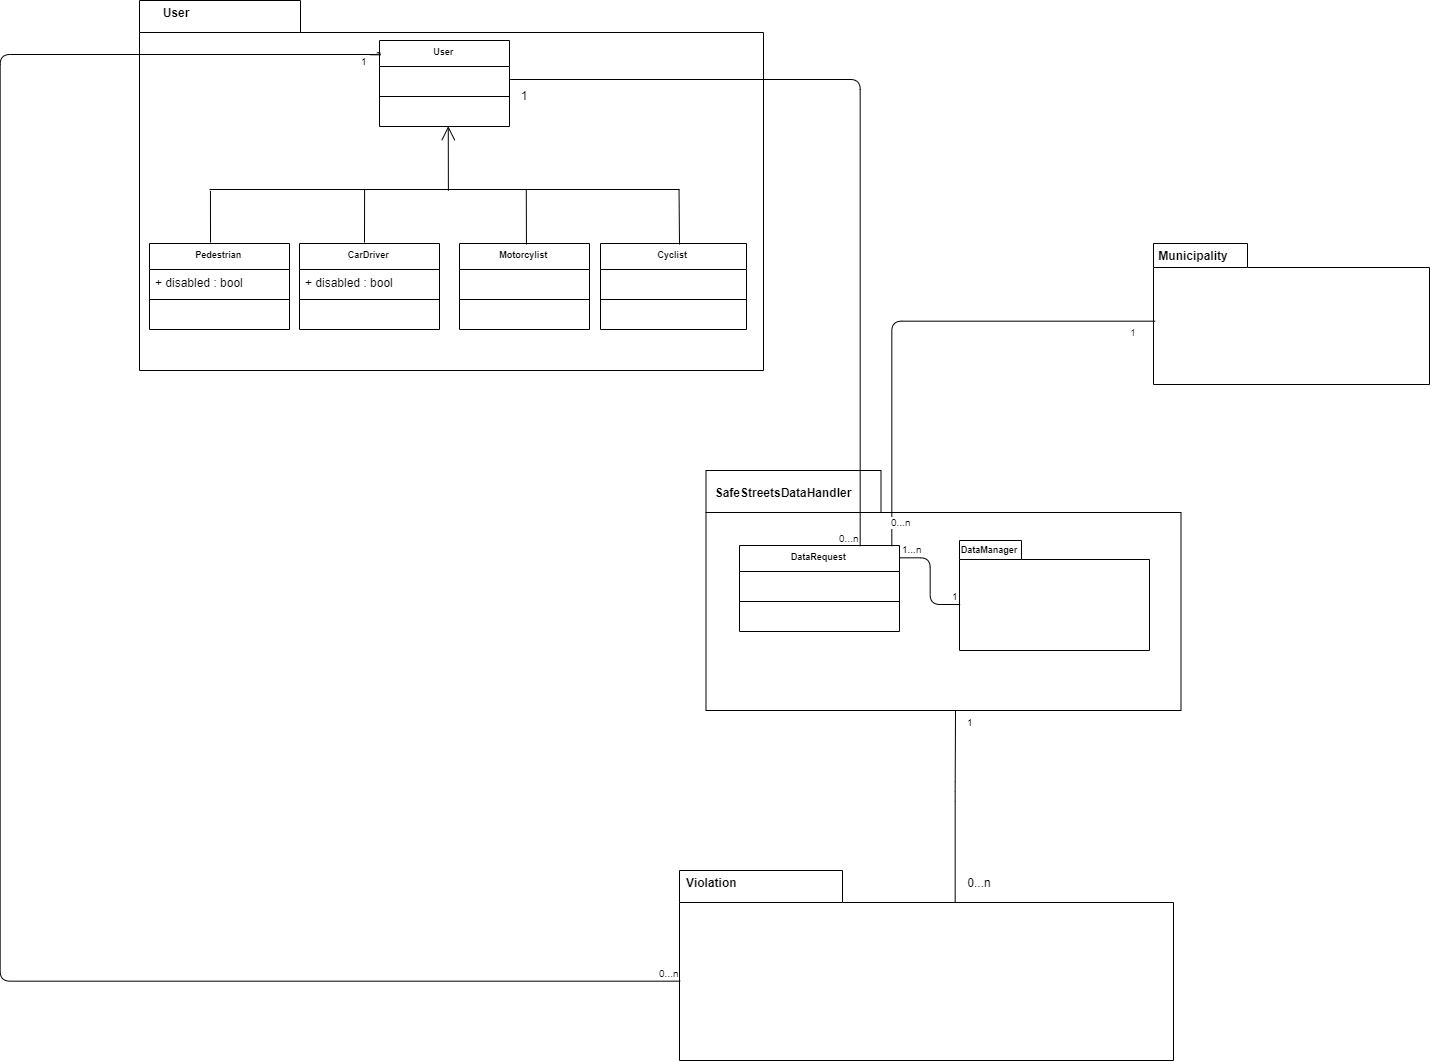
\includegraphics[scale=0.332]{UML users v1.0.png}
	\centering
	\caption{User class diagram}
\end{figure}
\FloatBarrier

\newpage
This is the violation class diagram:
\begin{figure}[h
]
	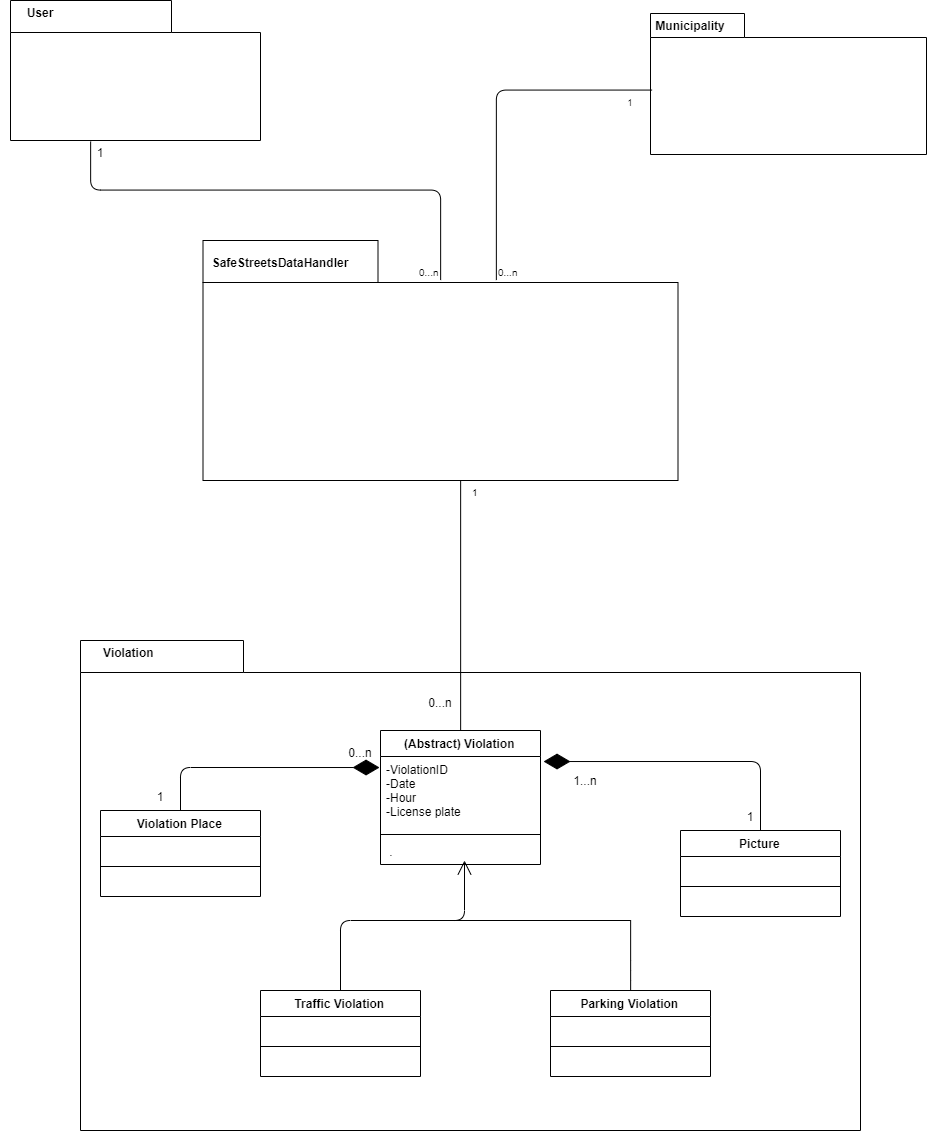
\includegraphics[scale=0.35]{UML violation v1.1.png}
	\centering
	\caption{Violation class diagram}
\end{figure}
\FloatBarrier

\newpage
\subsubsection{State charts }
Here you can find a state chart diagram of the system:

\begin{figure}[h
]
    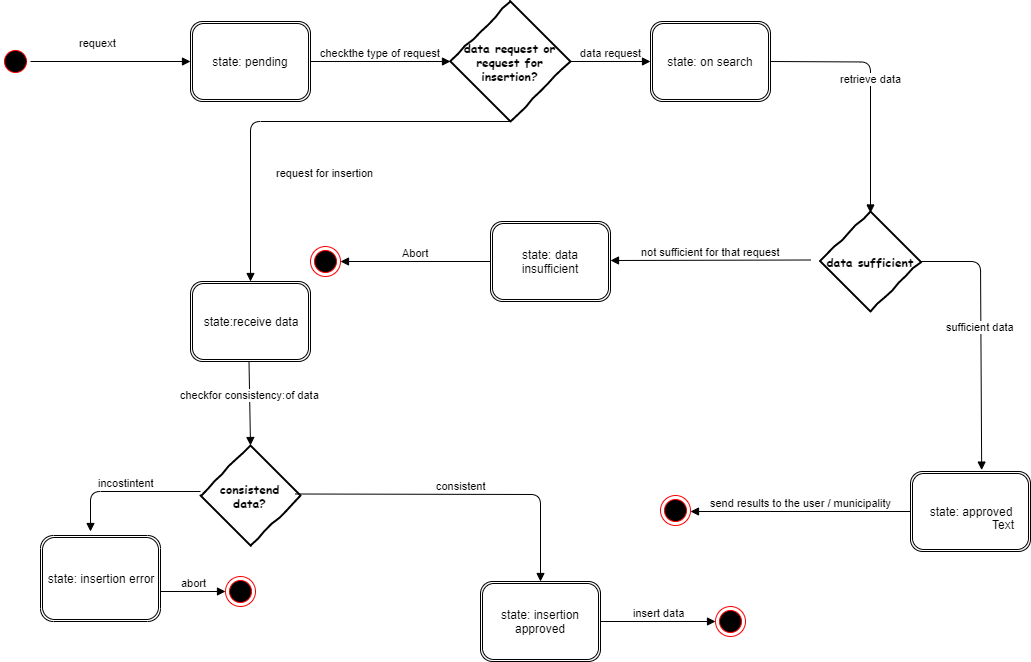
\includegraphics[scale=0.45]{State_chart.png}
	\centering
	\caption{System State chart diagram}
\end{figure}
\FloatBarrier


\subsection{Product functions}
In this section there is a description of the main functions that the system will make available to the final user.\\
These functions are the following:
\begin{itemize}
	\item \textbf{Report of a violation:} Safestreets allows the user to report a violation.This function must permit the user to take a picture directly and only from the application. It must also allow to insert the hour and the date. The street where the violation occur can be detected automatically or manually. In the first case the user decides that he/she wants to be localized through the GPS coordinates and in the last case the user must insert the street and the city manually into the application. It's very important to remark the important fact that the way in which the user wants to insert the street is only a choice of the private user.
	\item \textbf{Get the list of most dangerous streets: }
	The most dangerous streets are the ones with the highest violations and they can be retrieved specifying the maximum number of streets that the request has to show. \\
This function must also allow the user to insert the city of which he/she wants to know the dangerous roads and also a distance (expressed in kilometres). This function will provide a map with the dangerous streets highlighted. This function must take into consideration only the streets whose distance is less or equal to the one specified in the request by the user. 
	\item \textbf{Send a request to obtain suggestions to make the streets safer:}
	This function is only designed for the municipalities. In this case the municipality has to insert the place about which it wants to have suggestions. The system will return a list containing on one side the problem and on the other side a possible solution to overcome it. Obviously, the list is not static but it will be updated over time thanks to the reported violations.
	\item \textbf{The user send a request to know where to park his/her vehicle in a safe area:}
	This function allows the user to explicitly ask the system to suggest places where to park his/her vehicle in a secure way. 
The user must specify how far he/she wants to park from his/her position or from a position given as an input. The system will not guarantee the fact that in the proposed place there will be at least one parking lot but it only will suggest which roads are considered more secure than others to do so.
	\item \textbf{The user will receive the suggested areas where to park:}
	After having requested the safest areas where to park, the system will provide them to the user in a map form. In this map there will be highlighted the streets considered more secure than the others in the specified area given by the user as input.

\end{itemize}
\subsection{User characteristics}
In this subsection there is a description of the application users and an analysis of their needs. We will categorize the people who use the app in order to understand their necessities in a better way.\\
\textbf{\\Description of the users of the app:\\}
The user of the app can be divided in a first categorization which is the following:
\begin{itemize}
	\item Private user;
	\item Municipality.
	\item Authorities.\\
\end{itemize}
It is very important to say that the authorities are the only ones will not directly use the Safestreets system. They will be informed of the reports of violations by the municipality. The municipality is the entity which will receive all the reports and then it will forward them to the authorities. This choice is due to the fact that the authorities are part of the municipality, which manages them and Safestreets must not change the way in which the authorities are managed and organized internally. \\ \\
\textbf{Description of the private users: }\\ 
It is possible to divide again the private users in other classes. For every class there will be a different concept of dangerousness.
\begin{itemize}
	\item Pedestrians;
	\item Motorists;
	\item Motorcyclists;
	\item Cyclists.
\end{itemize}
A private user can be also a disabled person belonging to the pedestrians category or to the car drivers one (We suppose that it's rare that a person with motor disabilities drives a bicycle or a motorbike). Because of this fact these type of users will require a different type of service and a different concept of dangerousness. There are a lot of things that are not dangerous for non-disabled people and on the contrary others which are. We can make some brief examples: \\ \\
\textbf{1)} Streets which are not equipped with facilities for disabled pedestrians are for sure dangerous than for a non-disabled one.\\ \\
\textbf{2)} Streets with no parking lots for disabled can become impracticable for disabled car drivers. Maybe he/she could not have enough space for a wheelchair in a non-disabled car park. Instead for non-disabled ones this aspect does not generate any problem for sure. \\ \\
For example they will have information about cars parked in a handicap parking area or on ramps for disabled people.\\
All the private users are supposed to have downloaded the app from the store,to have done the sign-up entering all the mandatory data and finally to have accepted all the permissions.\\
The private user, according to his/her category, will take advantage of a different type of service.\\
A car driver, for example, will have information about parking lots or parking violation, that is not required in a biker service.\\
A cyclist will have informations about bicycle paths, while pedestrians will have detailed data about sidewalks or pedestrian crossing, with all the possible violations related to them. The location of the pedestrian crossings and of the bicycle paths must be provided by the municipality.  \\
Furthermore, the application can encounter:
\begin{itemize}
	\item Users that have downloaded the app but that haven't already signed-up in the system;
	\item Users that have already signed-up the system but that haven't logged-in yet. Users logged-out from the system belong to this category;
	\item Users also logged-in the system.\\
	
\end{itemize}

 



\subsection{Assumptions, dependencies and constraints}
\subsubsection{Domain assumptions }
\begin{itemize}
	\item $[\textbf{D1}]$: The user is supposed to submit a correct e-mail.
	\item $[\textbf{D2}]$: The user creates one and only one account.
	\item $[\textbf{D3}]$: Every municipality which has an account on the system certifies its own account as valid.
	\item $[\textbf{D4}]$: The GPS signal has a relative error of 10 meters.
	\item $[\textbf{D5}]$: The physical memory of SafeStreets database where the data about violations and streets is stored is persistent.
	\item$[\textbf{D6}]$: The user allows the app to have access to his/her position and the camera of his/her device.
	\item $[\textbf{D7}]$: The internet connection has to be enabled when the app needs it.
	\item $[\textbf{D8}]$: The municipality must provide the reports (sent by the users) to the authorities automatically.
	\item $[\textbf{D9}]$: The email identifies uniquely a private user.
	\item $[\textbf{D10}]$: The fiscal code identifies uniquely a person.
	\item $[\textbf{D11}]$: It is impossible that 2 roads that are in the same city have also the same name.
	\item $[\textbf{D12}]$: A street can be identified with its name and the city to which it belongs.
	\item $[\textbf{D13}]$: A disabled user belongs only to the pedestrians category or the car drivers one (Because we suppose that the users with motor disabilities rarely ride a bicycle or a motorbike).
	\item $[\textbf{D14}]$: SafeStreets has in its database a unique ID associated to a city (that only the municipality of that city knows).
	\item $[\textbf{D15}]$: The username identifies uniquely a user.
	
\end{itemize}
\subsubsection{Constraints }
\begin{itemize}
	\item  The system must treat the users' personal data in according to the GDPR regulation.
	\item The system will be designed and implemented for Android and IOS smartphones.
	\item The application will be available only in the Italian app stores.
\end{itemize}

\subsubsection{Dependencies }
\begin{itemize}
	\item The system will use the GPS services provided by the smart-phones.
	\item The system will use the internet services offered by the smart-phones.\\
\end{itemize}



\section{Specific Requirements}
\subsection{External Interface Requirements}
\subsubsection{User Interfaces}
\begin{itemize}
	\item\textbf{SafeStreet Interfaces}
	\begin{itemize}
		\item \textbf{SafeStreets Logo:}\\
		SafeStreets has a simple but explicative logo. It represents a street, because the main theme of the application concerns public roads. It also has a green tick, that represents the correct functioning and the safety of the streets.\\ 
		
	\begin{figure}[h]
	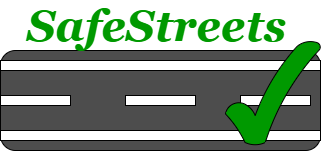
\includegraphics[scale=0.8]{Mockups/LogoSafeStreets.png}
	\centering
	\caption{SafeStreets Logo}
\end{figure}
\FloatBarrier


	\newpage
	
	\item \textbf{SafeStreets log-in page:}\\
	This is the page a user sees when he/she downloads the app and opens it for the first time or when he/she has done a log-out. In this page there is the possibility to log-in (inserting username and password) or to sign-up. The user can also recover his/her credentials using the function below the log-in button. When logged-in, the user will be redirected to the Home Page, that will be different for private users and authorities.
	\begin{figure}[h]
	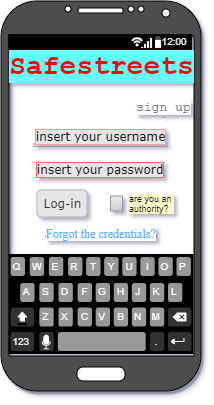
\includegraphics[scale=0.7]{Mockups/log in.png}
	\centering
	\caption{SafeStreets Log-in}
	\end{figure}
	\FloatBarrier
	
	
	\newpage
	
	\item \textbf{SafeStreets sign-up account choice:}\\
	
	Here the user can choose the type of account he/she wants to create. There is the account reserved to the municipality and the one available to a private user. By choosing one or the other, the user will be redirected to the second step of the sign-up.
	
	\begin{figure}[h]
	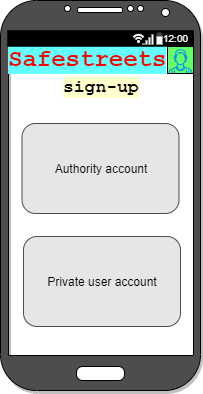
\includegraphics[scale=0.7]{Mockups/Account choice.png}
	\centering
	\caption{SafeStreets Account Choice}
	\end{figure}
	\FloatBarrier
	
	
	\newpage
	
	\item \textbf{SafeStreets private user sign-up:}\\
	
	This is the first part of the private user's  sign-up. Here the user has to put his/her username he/she will use in SafeStreets (that will also identify him uniquely) and the password, that has to comply the security policy. Then he/she can continue to the second part of the registration.
	\begin{figure}[h]
	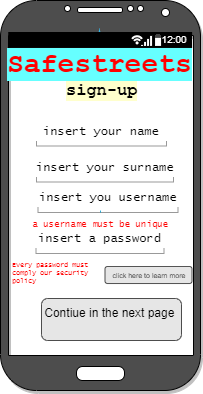
\includegraphics[scale=0.8]{Mockups/first sign up.png}
	\centering
	\caption{SafeStreets private user sign-up, first part}
	\end{figure}
	\FloatBarrier
	
	\newpage
	
	
	
	\item \textbf{SafeStreets private user sign-up (second part):}\\
	
	This is the second and last part of the private user's sign-up in the SafeStreets platform. Here the user has to fill the fields with his/her personal e-mail and his/her FC. Furthermore he/she has to choose  which category he(she belongs to (car driver, cyclist, motorcyclist, pedestrian, and so on) and he/she can also indicate if this account will be created for a disabled person or not. Finally he/she can add the ID of his/her driving license if he/she drives a vehicle that needs it (It's not mandatory). After doing that the sign-up is complete and the user will be redirected to the log-in page.
	
	\begin{figure}[h]
	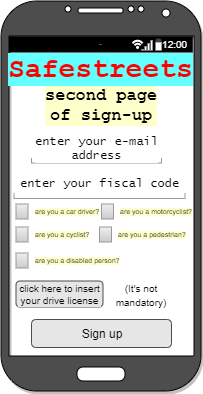
\includegraphics[scale=0.8]{Mockups/second sign up.png}
	\centering
	\caption{SafeStreets private user sign-up, second part}
	\end{figure}
	\FloatBarrier
	
	\newpage	
	
	
	
	
	\item \textbf{SafeStreets municipality sign-up:}\\
	If the user has chosen the municipality sign-up he/she will be redirected here. The authorities must indicate the city of their competence and must insert an ID code to prove that they have the authorization to represent the municipality. Then they have to insert a username and a password, in the same way as explained for private users. Then they will be redirected to the log-in page.
	
	\begin{figure}[h]
	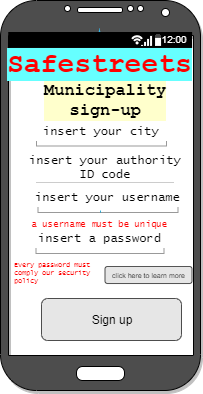
\includegraphics[scale=0.8]{Mockups/Municipality sign-up.png}
	\centering
	\caption{SafeStreets Municipality sign-up}
	\end{figure}
	\FloatBarrier
	
	\newpage
	
	
	
	
	
	\item \textbf{SafeStreets Private User's Home Page:}\\


		
	This is the Home Page reserved to private users. Its functions are very easy to understand and they are: the possibility to report a violation to the system, the chance to see which are the most reported streets in a selected area, the possibility to see the condition (in terms of safety) of a selected street, parking lot or area. Finally there is also the log-out button and the accessibility button, that allows the user to change his/her category.

	
	
	\begin{figure}[h]
	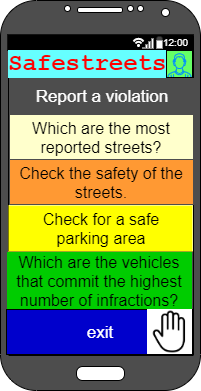
\includegraphics[scale=0.8]{Mockups/main functionalities.png}
	\centering
	\caption{SafeStreets Private Users' Home Page}
	\end{figure}
	\FloatBarrier
	
	\newpage	
	
	
	\item \textbf{SafeStreets Private User's Violation report:}\\

	This is the first function presented in the Home Page. Here the user can report a violation that he/she has seen. The first field to fill is the one that allows the user to describe the violation, indicating the type of violation that he/she has seen (for example motorcycle parking areas occupied by cars, or traffic accidents, and so on). Then he/she has to indicate the date and the hour of the violation. Furthermore a user has to indicate (manually or with GPS signal) the street and the city of the violation and finally he/she can take a photograph of the violation (this is mandatory).
	
	\begin{figure}[h]
	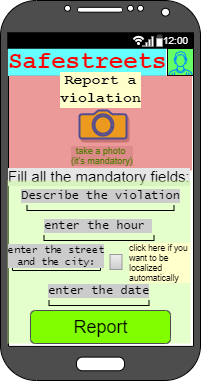
\includegraphics[scale=0.8]{Mockups/Report a violation.png}
	\centering
	\caption{SafeStreets Violation Reporting interface}
	\end{figure}
	\FloatBarrier
	
	\newpage
	
	
	
	
	
	
	\item \textbf{SafeStreets Most reported streets interface :}\\
		
	This interface allows the user to check which are the most reported streets in a city. The city can be inserted manually by the user or retrieved automatically by the system using the GPS signal of the user's smartphone. The user has to specify how many streets the list should be made up. Then he/she must submit the request and he/she will receive the list.
	
	
	\begin{figure}[h]
	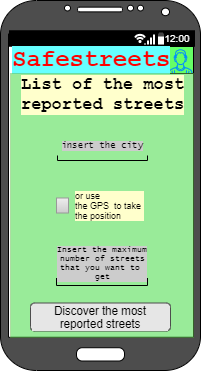
\includegraphics[scale=0.8]{Mockups/Most reported streets.png}
	\centering
	\caption{SafeStreets Most reported streets interface}
	\end{figure}
	\FloatBarrier
	
	\newpage		
	
	
	

	
	
	\item \textbf{SafeStreets safest streets interface :}\\
		
	Here the user can check which is the condition of a selected area. He/she can specify the street manually, inserting its name and the name of the city. The street can also be retrieved automatically by the system with the GPS signal of the user's smartphone. Then the user has to insert a radius (expressed in KM) within which the system will provide the condition of the contained streets, highlighting the safest and the most dangerous ones.
	\begin{figure}[h]
	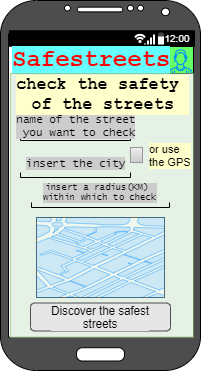
\includegraphics[scale=0.8]{Mockups/safest streets.png}
	\centering
	\caption{SafeStreets safest streets interface}
	\end{figure}
	\FloatBarrier
	
	\newpage		
	
	
	
	
	\item \textbf{SafeStreets safest parking areas :}\\
		
	The user can use this functionality to find the safest place where to park his/her vehicle. He/she has to specify his/her position, that can be done manually (inserting the name of the city and the street) or, as in the other functionalities, automatically (using the GPS signal of the smartphone). Then the user has to insert the maximum distance (expressed in kilometres) from the selected position to which he/she is willing to get. After have inserted all the needed information, the user will see the safest parking area where to go, highlighted differently from the less safe ones.
	\begin{figure}[h]
	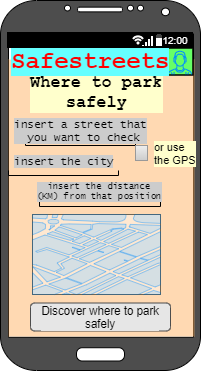
\includegraphics[scale=0.8]{Mockups/Park safely.png}
	\centering
	\caption{SafeStreets safest parking area interface}
	\end{figure}
	\FloatBarrier
	
	\newpage
	
	
	

	
	
	
	
	
	
	\item \textbf{SafeStreets User Category Change :}\\
	
	Here the user can change his/her category. There are some buttons, that represents a driver, a motorcyclist, a cyclist and a pedestrian. The user has to pick his/her new category.
	Then he/she can also indicate if the account will be used by a disabled person or not.
	
	\begin{figure}[h]
	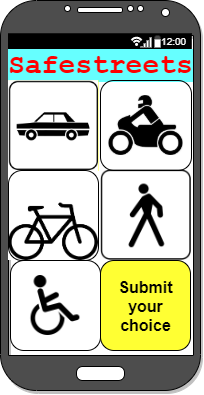
\includegraphics[scale=0.8]{Mockups/change type.png}
	\centering
	\caption{SafeStreets User Category change}
	\end{figure}
	\FloatBarrier
	
	\newpage
	
	
	
	
	
	\item \textbf{SafeStreets Municipality Home Page :}\\
	
	This is the Home Page reserved to the authorities. Here the municipality has the possibility to choose between four functionalities:
	three are structured in the same way of the ones designed for the private users and it's the possibility to check the most reported streets. The third is the one to check the conditions of a selected area. The interfaces for the requests are the same than the ones for the users. The municipality also has the possibility to do a request to obtain suggestions in order to improve the quality of their service and, so, the safety of the city. 
	
	\begin{figure}[h]
	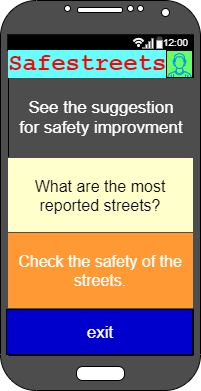
\includegraphics[scale=0.8]{Mockups/Municipality main functionalities.png}
	\centering
	\caption{SafeStreets Municipality Home Page}
	\end{figure}
	\FloatBarrier
	
	\newpage
	
	
	
	
	
	\item \textbf{SafeStreets Municipality suggestions request :}\\
	
	Here the municipality can make a request in order to discover which are the suggestions provided by SafeStreets to enhance the safety of the city. The authorities have to insert the name of the city, or provide it using the GPS signal of their device.
	
	\begin{figure}[h]
	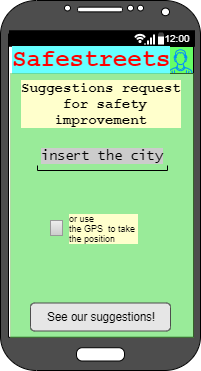
\includegraphics[scale=0.8]{Mockups/Request for safety improvements.png}
	\centering
	\caption{SafeStreets Municipality Suggestions Request}
	\end{figure}
	\FloatBarrier
	
	\newpage
	
	
	
	After having submitted the information, the municipality will receive the suggestions provided by SafeStreets concerning the indicated city. The data is retrieved by SafeStreets mining the information received by the users with their reports.
	
	
	\begin{figure}[h]
	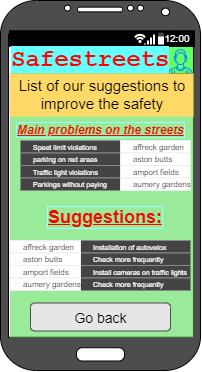
\includegraphics[scale=0.95]{Mockups/List of suggestions.png}
	\centering
	\caption{SafeStreets Municipality Suggestions List}
	\end{figure}
	\FloatBarrier
	
	\newpage
	
		
		
	\end{itemize}

		
		
	\end{itemize}
	
\subsubsection{Hardware Interfaces }
The system doesn't offer any kind of hardware interface to the user. In fact the user can use the application simply thanks to his/her phone.
\subsubsection{Software interfaces }
The system offers its service through the use of the following software interfaces:\\ \\
\textbf{Operating systems:\\ }
The system will have to be designed for the most common smart-phones operating system: 
	
\begin{itemize}
	\item Android 
	\item IOS
\end{itemize}
	
\subsubsection{Communication interfaces }
Each smart-phone that will use Safestreets will communicate with the servers thanks to the HTTPS protocol. Also the databases will communicate with the server using the same protocol. We've chosen this protocol because thanks to it, it is possible to obtain a secure connection between nodes. Furthermore it is a very commonly used protocol for the connections over internet.
\subsection{Functional Requirements:}
\subsubsection{Use case diagrams: }
Use case diagrams are very important because they allow the reader to understand the flow of events between actors and the system itself. We have done two different use case diagrams to make them more explanatory and less confusing.

\begin{figure}[h]
	\textbf{The first diagram:\\ \\}
	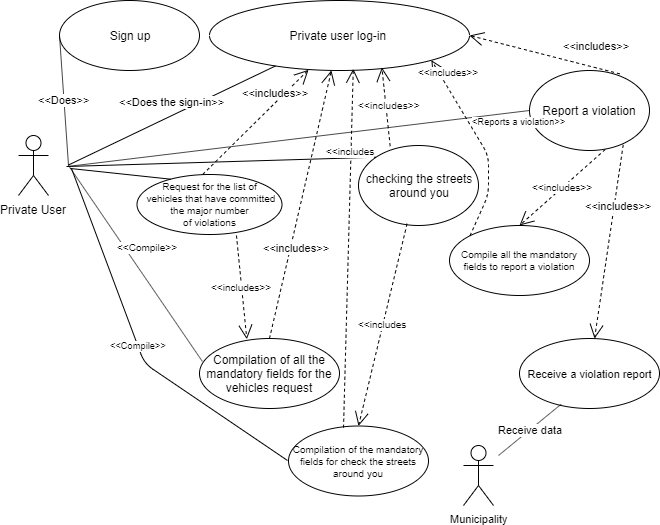
\includegraphics[scale=0.65]{use case diagrams/use case diagrams.png}
	\centering
	\caption{First use case diagram}
\end{figure}
\FloatBarrier

\begin{figure}[h]
	\textbf{The second diagram:\\ \\ }
	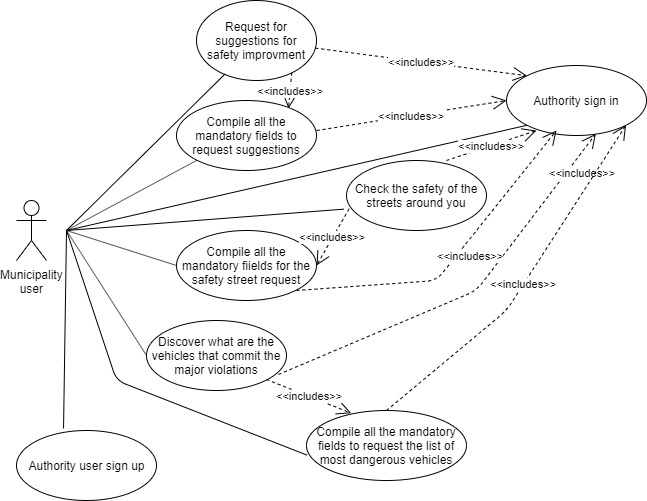
\includegraphics[scale=0.65]{use case diagrams/use-case2.png}
	\centering
	\caption{Second use case diagram}
\end{figure}
\FloatBarrier

\subsubsection{Scenarios}
\begin{center}
\textbf{From the private user point of view:}
\end{center}

\paragraph{Scenario 1:}Luigi is a middle-aged man who lives in a very busy area of Milan. This district is very known to be a zone with a strong lack of parking. People usually park their vehicles in illegal zones.
Because of this, he has found  cars parked in front of his home gate several times. He has called the municipality and the authorities many times and now he is fed up about this situation. He usually calls the authorities with his phone but this process takes a lot of time because the telephone line is always busy. He would like the authorities to have a better communication channel.\\Luckily he has downloaded an application called Safestreets. He has read in the description the fact that the application allows a user to report a violation via smart-phone.\\
Thanks to this mobile application he is now able to save time in reporting violations. Furthermore, he has observed that  the authorities have started to check more frequently even without any report (because of the Safestreets suggestions to the municipality that have suggested to authorities to check more frequently).
\paragraph{Scenario 2:}Giovanni lives very close to the place where he/she works but he usually goes to work by car even if he would like to go there by bicycle. The problem is that the zone is very busy and unfortunately accidents involving cyclists happen very often. Because of this, he does not feel like taking the risk.
He notices an interesting application on the market called Safestreets. He is particularly interested in the function which suggest the safest streets around the user from a point of view of the category in which the user has signed-up. This interest is caused by the idea of ​​being able to choose a route that minimizes the danger of making an accident against a car taking in consideration the suggested streets given by the application.\\
Now, he is finally able to go to work by bicycle in a secure way.
\paragraph{Scenario 3:}Andrea is a disabled person who strolls very often in his district. Unfortunately not all the roads are equipped with facilities for disabled people and also a lot of people park their cars there.\\
He has downloaded the application which suggests him the streets which are the most secure to be travelled for a person with his problem. The app allows Andrea to avoid roads where it is more probable to have cars parked on disabled facilities. When he sees a violation he can report it to the authorities. Thanks to this feature Andrea is able to report violations, to do his strolls in the city almost in an autonomous way. 
\paragraph{Scenario 4:} An employee of an insurance has the task of understanding which are the most dangerous areas of Milan in order to change the price of insurance. He does not know where to find the data necessary to do this task.Furthermore it has just been decided by the boss that funding a research would be too costly.\\
Fortunately the insurance company has just downloaded the Safestreets applications which can be used to retrieve dangerous areas. Thanks to Safestreets the company saved a lot of money by doing a free data search.\newpage
\begin{center}
	\textbf{From the municipality point of view:}
\end{center}
\paragraph{Scenario 5:} The municipality of Milan is worried about the safety of the streets in a particular zone. The zone that we are considering is full of pedestrian crossings and unfortunately a lot of cars exceed the speed limit constantly making the street very dangerous for pedestrians. The municipality to improve the safety taking in consideration various projects.\\
It has recently discovered that there exist the application Safestreets that helps the municipalities to do changes in the streets to improve the safety. The municipality has taken in account the suggestions and it has noticed that the projects now have improved and become more detailed.

\subsubsection{Use Cases}

\begin{longtable}{| p{3 cm} | p{10 cm} |} 
\hline



\textbf{ID code}   & Use Case 1\\ \hline
\textbf{Name}	& Private user sign-up \\ \hline
\textbf{Actor}     & Private user	 \\ \hline
\textbf{Preconditions} & 
\begin{itemize}
	\item The private user has downloaded SafeStreets on his/her device. 
	\item The private user has not already created an account on SafeStreets.
\end{itemize} 
     \\ \hline
     
\textbf{Events flow} & 
\begin{enumerate}
	\item The private user opens Safestreets;
	\item The system shows the private user the log-in page;
	\item The private user selects sign-up;
	\item The system asks the user to choose between private account and municipality account;
	\item The private user chooses private account;
	\item The system shows the user the first page of the private account registration;
	\item The private user inserts a username;
	\item The private user inserts a password;
	\item The private user submits his/her data;
	\item The system checks the correctness of this first part of the sign-up;
	\item The system shows the user the second part of the registration;
	\item The user inserts his/her personal e-mail;
	\item The user inserts his/her FC;
	\item The user indicates his/her category;
	\item The user indicates if the account will be used by a disabled person;
	\item If he/she is a car driver or a motorcyclist, the user can insert his/her driving license;
	\item The user submits these other data;
	\item The system checks the new data;
	\item The system sends the user an e-mail to confirm the registration;
	\item The user confirms the sign-up;
\end{enumerate} \\ \hline
\textbf{Postconditions} & 
\begin{itemize}
\item The system stores the private user's account data in its database;
\item The user has a personal account and can do the log-in, accessing the functionalities of SafeStreets.
\end{itemize} \\ \hline

\textbf{Exceptions} & 
\begin{itemize}
	\item The private user inserts an email that is already associated to an account;
	\item The private user inputs a password that isn't valid because it doesn't comply the security policy;
	\item The private user inserts a FC already associated to an account.;
	\item The private user inserts personal data that don't match with the FC;
	\item The user doesn't specify his/her category;
\end{itemize} 
							
For all these exceptions: The system shows the user an error message and the events restart from the first page of private user registration (Event 6).


\begin{itemize}
\item The user selects the login button inserting not existing credentials.
\end{itemize} 
The system shows the user an error message and the user will be redirected in the log-in page (Event 2).

\\ \hline
							

\end{longtable}

\newpage

\begin{longtable}{| p{3 cm} | p{10 cm} |} 
\hline

\textbf{ID code} & Use Case 2 \\ \hline
\textbf{Name} & Municipality sign-up \\ \hline
\textbf{Actor} & Municipality \\ \hline
\textbf{Precondition} & 
\begin{itemize}
\item The municipality has downloaded Safestreet on a smartphone.
\item The municipality doesn't already have an account on SafeStreets.
\end{itemize} \\ \hline
\textbf{Events flow} &
\begin{enumerate}
\item The municipality opens SafeStreets;
\item The system shows the municipality the log-in page;
\item The municipality selects sign-up;
\item The system asks the municipality to choose between private account and municipality account;
\item The municipality chooses municipality account;
\item The system shows the municipality the account registration page;
\item The municipality inserts the city of its competence;
\item The municipality inserts its unique ID code;
\item The municipality inserts a username;
\item The municipality inserts a password;
\item The municipality submits its data;
\item The system checks the correctness of the data inserted by the municipality;
\item The system automatically confirms the registration.
\end{enumerate} \\ \hline
\textbf{Postconditions} &
\begin{itemize}
\item The system stores the data about the new municipality account on its database;
\item The municipality now has an account and can log-in, accessing the municipality functionalities of SafeStreets.
\end{itemize} \\ \hline


\textbf{Exceptions} & 
\begin{itemize}
	\item The municipality inserts a password that isn't valid because it doesn't comply the security policy;
	\item The municipality inserts an ID code already associated to an account;
	\item The municipality inserts a wrong ID code. The ID code is considered wrong if and only if it doesn't match the code corresponding to its city in SafeStreets database.
	
	\item The municipality inserts a city that has already an account associated to it;
\end{itemize} 
	
							
For all these exceptions: The system shows the user an error message and the events restart from the municipality registration page (Event 6).


\begin{itemize}
\item The municipality selects the login button inserting not existing credentials.
\end{itemize} 
The system shows the user an error message and the user will be redirected in the log-in page (Event 2).
\\ \hline

\end{longtable}

\newpage

\begin{longtable}{| p{3 cm} | p{10 cm} |} 
\hline


\textbf{ID code} & Use Case 3 \\ \hline
\textbf{Name} & Log-in \\ \hline
\textbf{Actor} & User (private or municipality) \\ \hline
\textbf{Precondition} & 
\begin{itemize}
\item The user has downloaded the application;
\item The user has already done the sign-up.
\end{itemize} \\ \hline

\textbf{Events flow} & 
\begin{enumerate}
\item The user opens SafeStreets;
\item The system shows the user the log-in page
\item The user fills the form inserting his/her personal credentials;
\item The user submits the credentials tapping on the log-in button;
\item The system checks the correctness of the credentials.
\end{enumerate} \\ \hline

\textbf{Postconditions} & 
\begin{itemize}
\item The user is logged-in, so he/she is redirected to the Home Page and is able to use SafeStreets with its functionalities, that are different for private and municipality accounts. 
\end{itemize} \\ \hline

\textbf{Exceptions} &
\begin{itemize}
\item The user inserts wrong or not existing credentials;
\end{itemize}
The system sends notifies the user with an error message and redirects him/her to the log-in page (Event 2).
\\ \hline

\end{longtable}

\newpage


\begin{longtable}{| p{3 cm} | p{10 cm} |} 
\hline

\textbf{ID code} & User Case 4 \\ \hline
\textbf{Name} & Private User Violation Report \\ \hline
\textbf{Actor} & Private user and Municipality\\ \hline
\textbf{Preconditions} & 
\begin{itemize}
\item The user has logged into SafeStreets.
\end{itemize} \\ \hline
\textbf{Events flow} &
\begin{enumerate}
\item The private user selects "Report a violation" in his/her Home Page;
\item The system shows the user the report page;
\item The user takes a photo and uploads it;
\item The user describes the violation, indicating in particular the type (parking, traffic, etc.);
\item The user inserts the date and the hour of the violation.
\item The user inserts manually the place where the violation has occurred or , alternatively, uses his/her GPS signal to provide it automatically.
\item The user submits his/her report.
\item The system checks the correctness of the report;
\item The system retrieves the license plate with an algorithm from the photograph and then stores the data about the violation in its database;
\item The system sends the report to the municipality;
\item The municipality receives the report and forwards it to the authorities.
\end{enumerate} \\ \hline
\textbf{Postconditions} & 
\begin{itemize}
\item The system database now contains the information about the violation;
\item The authorities now have the report.
\end{itemize} \\ \hline
\textbf{Exceptions} & 
\begin{itemize}
\item The system can't manage to retrieve the license plate from the picture;
\item The user doesn't put complete data about the violation; 
\end{itemize}
In this cases the system sends an error message and redirect the user to the report page (Event 2). \\ \hline
\end{longtable}

\newpage

\begin{longtable}{| p{3 cm} | p{10 cm} |} 
\hline

\textbf{ID code} & Use Case 5 \\ \hline
\textbf{Name} & Most reported streets \\ \hline
\textbf{Actor} & User (private or municipality) \\ \hline
\textbf{Preconditions} & 
\begin{itemize}
\item The user has logged into SafeStreets.
\end{itemize} \\ \hline
\textbf{Events flow} & 
\begin{enumerate}
\item The user selects "Which are the most reported streets?" in his/her Home page;
\item The system shows the user the most reported streets interface;
\item The user inserts, manually or automatically (with GPS signal), the city he/she wants to check;
\item The user must specify how many streets the system must provide him;
\item The user submits his/her request;
\item The system checks the correctness of the request;
\item The system provides the list of the most reported streets.
\end{enumerate} \\ \hline
\textbf{Postconditions} & 
\begin{itemize}
\item The user will see the list of the most reported streets.
\end{itemize} \\ \hline
\textbf{Exceptions} &
\begin{itemize}
\item The user provides a non existing city name;
\item The user provides a non valid number of streets he/she wants to receive;
\end{itemize}
The system sends an error message and redirects the user to the most reported streets request interface (Event 2). \\ \hline

\end{longtable}

\newpage

\begin{longtable}{| p{3 cm} | p{10 cm} |} 
\hline

\textbf{ID code} & User Case 6 \\ \hline
\textbf{Name} & Checking the safety of an area \\ \hline
\textbf{Actor} & User (private or municipality) \\ \hline
\textbf{Preconditions} & 
\begin{itemize}
\item The user is logged into SafeStreets.
\end{itemize}\\ \hline

\textbf{Events flow} &
\begin{enumerate}
\item The user selects "Check the safety of the streets" in the Home Page;
\item The system show the user the interface to do a street check request;
\item The user specifies the street and the city to check (manually or automatically with GPS signal);
\item The user indicates how far from the indicated point the system has to provide the information about the safety of the area;
\item The user submits the request to the system;
\item The system checks the correctness of the request;
\item The system provides the map with the requested area highlighted. 
\end{enumerate} \\ \hline
\textbf{Postconditions} & 
\begin{itemize}
\item The user will see a map of the indicated area with the safest and the most dangerous streets highlighted in a different way.
\end{itemize} \\ \hline
\textbf{Exceptions} &
\begin{itemize}
\item The user provides a non existing street or city;
\item The user indicates a non valid radius;
\end{itemize}
The system sends an error message and redirects the user to the streets safety request interface (Event 2). \\ \hline



\end{longtable}


\newpage

\begin{longtable}{| p{3 cm} | p{10 cm} |} 
\hline

\textbf{ID code} & Use Case 7 \\ \hline
\textbf{Name} & Check the safety of a parking area \\ \hline
\textbf{Actor} & Private user \\ \hline
\textbf{Preconditions} &
\begin{itemize}
\item The user is logged into SafeStreets.
\end{itemize} \\ \hline

\textbf{Events flow} &
\begin{enumerate}
\item The user selects "Check for a safe parking area" in the Home Page;
\item The system shows the user the page to do the request for safe parking areas;
\item The user specifies the street and the city near which to check (manually or automatically with GPS signal);
\item The user indicates how far from the indicated point the system has to provide parking areas;
\item The user submits the request to the system;
\item The system check the correctness of the request;
\item The system provides the map with the requested parking areas highlighted. 

\end{enumerate} \\ \hline

\textbf{Postconditions} &
\begin{itemize}
\item The user will see a map, provided by the system, that contains the parking areas in the zone requested by him, with the safest and the most dangerous ones highlighted with different colours.
\end{itemize} \\ \hline

\textbf{Exceptions} &
\begin{itemize}
\item The user provides a non existing street or city;
\item The user inserts a non valid distance from which to check;
\end{itemize}
For this exceptions the system sends to the user an error message and redirects him/her to the request page (Event 2). \\ \hline




\end{longtable}

\newpage



\begin{longtable}{| p{3 cm} | p{10 cm} |} 
\hline

\textbf{ID code} & Use Case 8 \\ \hline
\textbf{Name} & Suggestions for municipality \\ \hline
\textbf{Actor} & Municipality \\ \hline
\textbf{Preconditions} &
\begin{itemize}
\item The municipality is logged into SafeStreets;
\end{itemize} \\ \hline

\textbf{Events flow} & 
\begin{enumerate}
\item The municipality user selects "See the suggestions for safety improvements" in the Home Page;
\item The system shows the municipality user the page to make the suggestion request;
\item The municipality user insert the city for which he/she wants to receive suggestions (with GPS signal or manually);
\item The user submits the request for the city of competence of his/her municipality;
\item The system checks the correctness of the request;
\item The system, with a data mining algorithm, retrieves useful information from the users' reports regarding that city and adds it to the information that it has from the municipality side;
\item The system sends the result of its research to the municipality user.
\end{enumerate} \\ \hline

\textbf{Postconditions} &
\begin{itemize}
\item The municipality will see a table showing the suggestion that the system has provided for their city. This table is structured to have on one side the problem reported by the users, and on the other side the solution provided by SafeStreets.
\end{itemize} \\ \hline

\textbf{Exceptions} &
\begin{itemize}

\item The municipality user provides a non existing city;
\end{itemize}
The system will send to the user an error message and will redirect him/her in the suggestions request page. \\ \hline

\end{longtable}

\newpage

\begin{longtable}{| p{3 cm} | p{10 cm} |} 
\hline

\textbf{ID code} & Use Case 9 \\ \hline
\textbf{Name} & Change of the user type \\ \hline
\textbf{Actor} & Private user \\ \hline
\textbf{Preconditions} &
\begin{itemize}
\item The user is logged into SafeStreets.
\end{itemize}\\ \hline

\textbf{Events flow} &
\begin{enumerate}
\item The user taps the accessibility button (represented with a hand) in the Home Page;
\item The system shows the user the interface for selecting his/her new type;
\item The user selects his/her new type and submits his/her selection by tapping it on the touch screen;
\item The system stores the new data about the user in its database;
\end{enumerate} \\ \hline

\textbf{Postconditions} &
\begin{itemize}
\item The system has the new information about the user's type in its database.
\end{itemize} \\ \hline

\textbf{Exceptions} & \\ \hline




\end{longtable}


\newpage

\begin{longtable}{| p{3 cm} | p{10 cm} |} 
\hline


\textbf{ID code} & Use Case 10 \\ \hline
\textbf{Name} & Log-out \\ \hline
\textbf{Actor} & User (private or municipality one) \\ \hline
\textbf{Preconditions} & 
\begin{itemize}
\item The user is logged into SafeStreets.
\end{itemize}  \\ \hline

\textbf{Events flow} & 
\begin{enumerate}
\item The user taps the log-out button in the Home Page;
\item The system asks the user for the confirm of the log-out;
\item The user confirms the log-out.
\end{enumerate} \\ \hline

\textbf{Postconditions} & 
\begin{itemize}
\item The user will be logged out from SafeStreets and will be redirected to the log-in page.
\end{itemize} \\ \hline

\textbf{Exceptions} & \\ \hline



\end{longtable}

\newpage

\subsubsection{Sequence Diagrams}
\begin{itemize}

\item The first sequence diagram represents the registration process. The actors are the user (municipality or private one) and the system. 

\begin{figure}[h]
	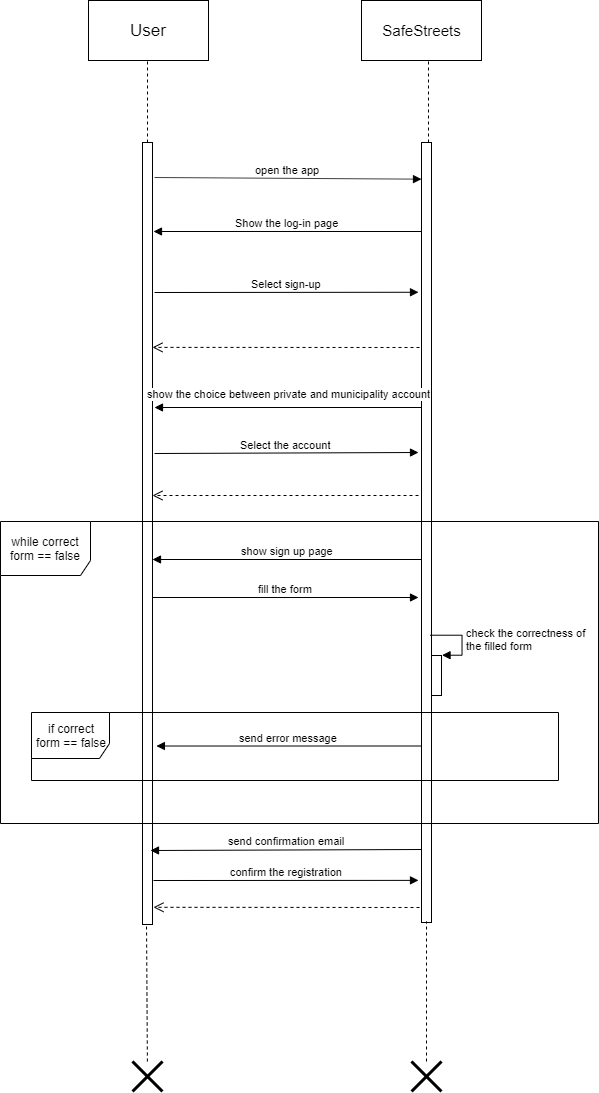
\includegraphics[scale=0.365]{Sequence Diagrams/Sequence diagram sign-up.png}
	\centering
	\caption{First Sequence Diagram}
\end{figure}
\FloatBarrier 

\newpage



\item The second sequence diagram represents the log-in process. The actors are the user (municipality or private one) and the system. 

\begin{figure}[h]
	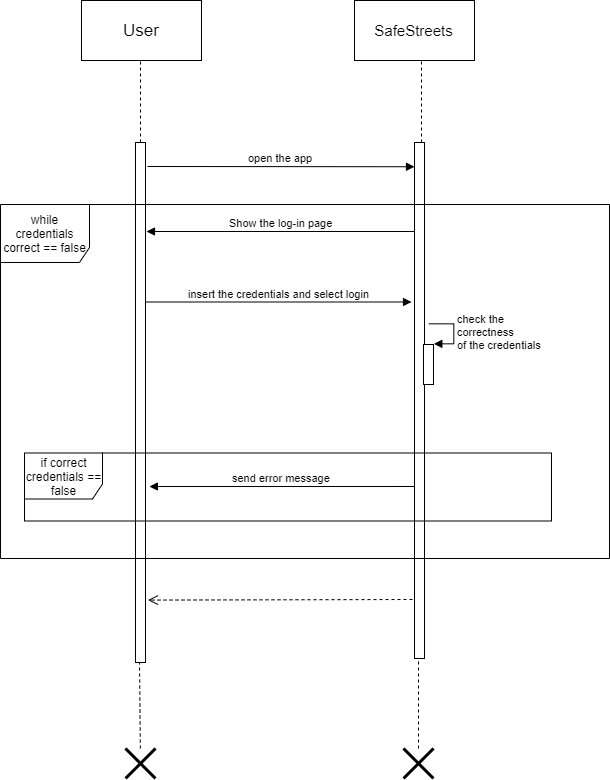
\includegraphics[scale=0.51]{Sequence Diagrams/Sequence diagram log-in.png}
	\centering
	\caption{Second Sequence Diagram}
\end{figure}
\FloatBarrier

\newpage


\item The third sequence diagram represents the violation reporting process. The actors are the private user that sends it, the system and the municipality that receives it.

\begin{figure}[h]
	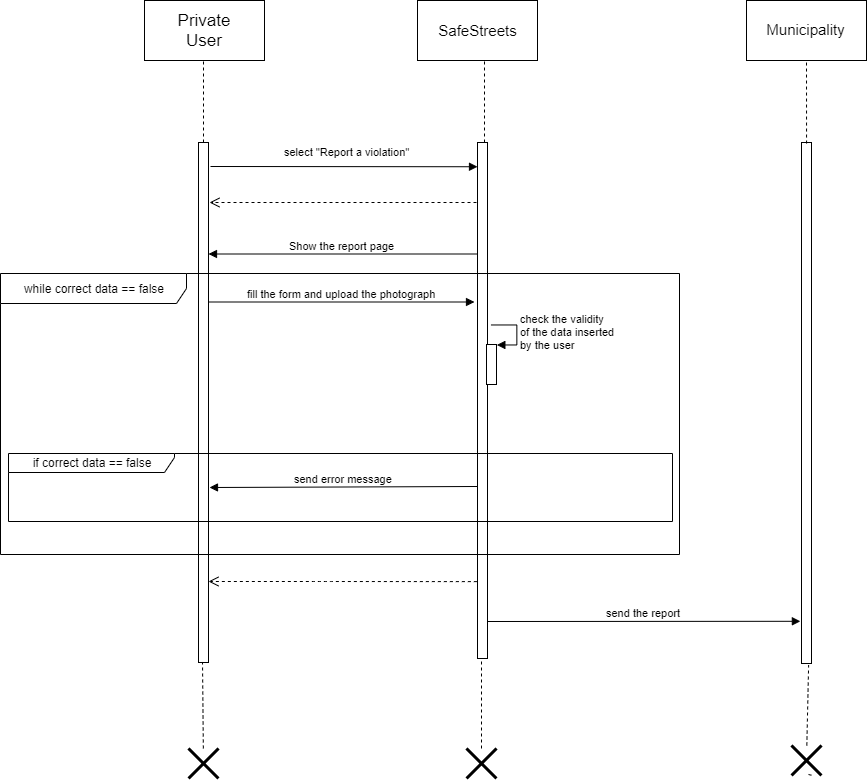
\includegraphics[scale=0.51]{Sequence Diagrams/Sequence diagram violation.png}
	\centering
	\caption{Third Sequence Diagram}
\end{figure}
\FloatBarrier  


\newpage


\item The fourth sequence diagram represents process to make a request to the system. The actors are the user (private and municipality) and the system. The private user uses this process to request for the safest parking areas, the condition of the streets, the most reported streets and the most reported vehicles, while the municipality can make the request for the most reported vehicles and streets, the condition of an area and to receive suggestions for improvements.

\begin{figure}[h]
	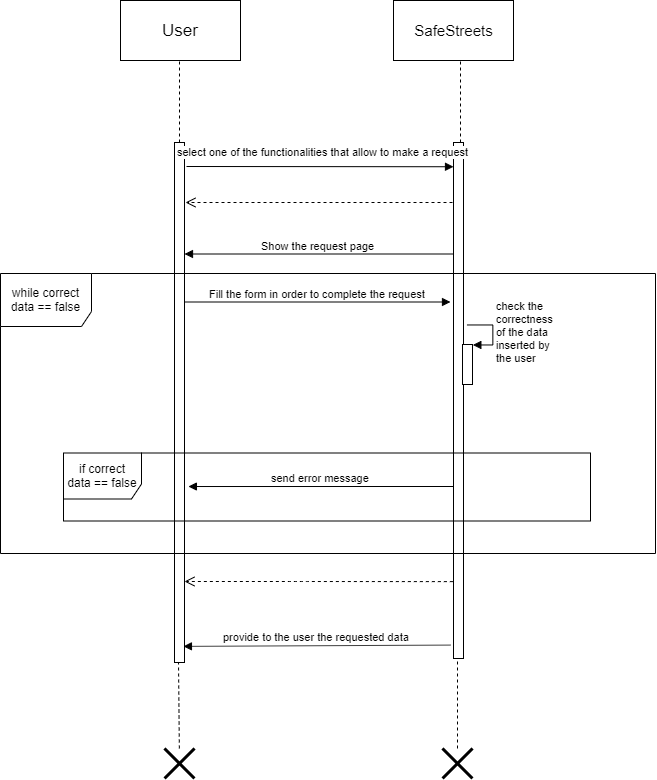
\includegraphics[scale=0.51]{Sequence Diagrams/Sequence diagram request.png}
	\centering
	\caption{Fourth Sequence Diagram}
\end{figure}
\FloatBarrier 


\newpage





\item The fifth and last sequence diagram represents the process for changing the category of the private user. The actors are the private user that wants to change his/her category and the system.

\begin{figure}[h]
	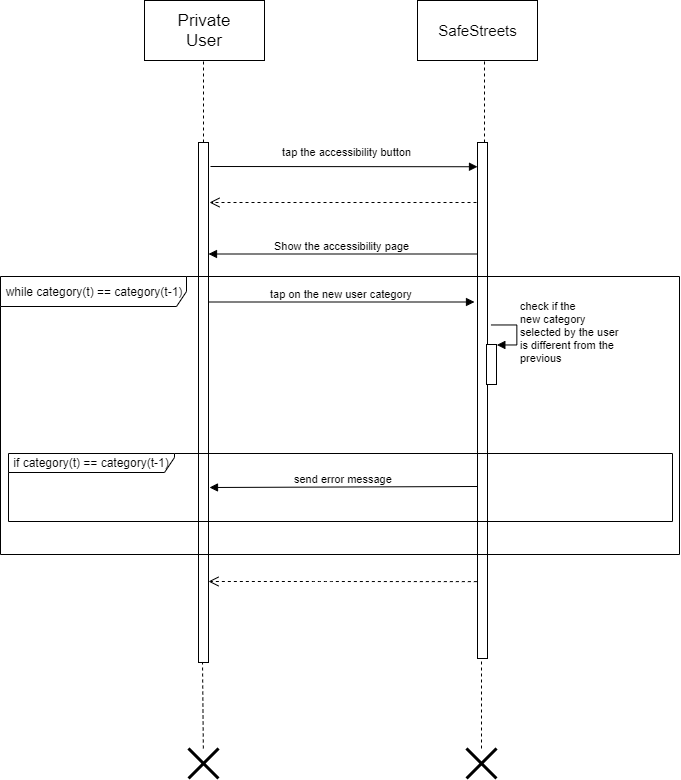
\includegraphics[scale=0.51]{Sequence Diagrams/Sequence diagram change category.png}
	\centering
	\caption{Fifth Sequence Diagram}
\end{figure}
\FloatBarrier 


\end{itemize}


\newpage

\subsubsection{Goal mapping on requirements}
\begin{itemize}
 \item $[G1]:$ The service allows the users to report a violation to the municipality:
 \begin{itemize}
 	\item $[R1]:$ The system must allow the user to take a picture.
 	\item $[R2]:$ The system must allow the user to indicate the street where the violation occurred.
 	\item $[R3]:$ The system must allow the user to indicate the hour and the date when the violation occurred.
 	\item $[R4]:$ The system must allow the user to insert a brief description of the violation.
 	\item $[R5]:$ The system can localize the user's position automatically (with GPS signal) as alternative to the manual insertion.
 	\item $[R6]:$ The system must allow the user to finally submit the report.
 	\item $[R7]:$ The system must run an algorithm to retrieve the license plate from the violation picture.
 	\item $[R8]:$ The chosen username must identify the private user uniquely.
 	\item $[R9]:$ The pictures must be taken only through the app camera and not imported from the device gallery in order to take photos in real time.
 	\item $[R10]:$: The system must store the report if it is correct.
 	\item $[R11]:$: The system must check if the reported street exists in reality.
 	\item $[R13]:$ The system must be able to retrieve users' position data from the GPS service of their smartphones.
 	\item $[D4]:$ The GPS signal has a relative error of 10 meters.
 	\item $[D5]:$ The physical memory of SafeStreets database where the data about violations and streets is stored is persistent.
 	\item $[D6]:$ The user allows the application to have access to his/her position and to the camera of his/her device.
 	\item $[D7]:$ The internet connection has to be enabled when the app needs it.
 	\item $[D8]:$ The municipality must provide the reports (sent by the users) to the authorities automatically.
 	\item $[D11]:$ It is impossible that two roads that are in the same city have also the same name.
 	\item $[D12]:$ A street can be identified with its name and the city to which it belongs.

 	
 \end{itemize}
 \item $[G2]:$ The service allows the users to have detailed informations about the violations and the streets safety.
 \begin{itemize}
 	\item $[R12]:$ The system must allow the user to insert the street around which he/she wants to check the safety.
 	\item $[R13]:$ The system must be able to retrieve users' position data from the GPS service of their smartphones.
 	\item $[R14]:$ The system must allow the user to insert the city to which the inserted street belongs.
 	\item $[R15]:$ The system must allow the user to insert a number representing the radius within which the system must provide the condition of the streets.
 	\item $[R16]:$ The system must return the  safest streets in a map form. These streets must be highlighted on the map.
 	\item $[R18]:$ The system must retrieve the information about the streets safety and the violation from its cloud database.
 	\item $[D4]:$ The GPS signal has a relative error of 10 meters.
 	\item $[D5]:$ The physical memory of SafeStreets database where the data about violations and streets is stored is persistent.
 	\item $[D6]:$ The user allows the application to have access to his/her position and to the camera of his/her device.
 	\item $[D7]:$ The internet connection has to be enabled when the app needs it.
 	\item $[D11]:$ It is impossible that two roads that are in the same city have also the same name.
 	\item $[D12]:$ A street can be identified with its name and the city to which it belongs.
 \end{itemize}
 
 
 
 \item $[G3]:$ Safestreets must send to the municipality suggestions to improve the safety of the streets whenever the municipality asks for them.
 \begin{itemize}
 \item $[R17]:$ The system must run a data mining algorithm to merge the information about the violations and the streets safety(retrieved from the Safestreets database and the Municipality one).
 \item $[R18]:$ The system must retrieve the information about the streets safety and the violation from its cloud database.
 \item $[R19]:$ The system must retrieve the information about violations from the Municipality external database.
 \item $[R20]:$ The system must use both data received by the users and by the municipality.
 \item $[R21]:$ The Data Mining API must create suggestions from the data sent by the system and analysed.
 \item $[R22]:$ The system must provide the suggestions created and dispatched by the Data Mining API to the Municipality.
 \item $[D5]:$ The physical memory of SafeStreets database where the data about violations and streets is stored is persistent.
 \item $[D7]:$ The internet connection has to be enabled when the app needs it.
 \end{itemize}
 
 
 \item $[G4]:$ The user (both private user and the municipality) must be able to authenticate into the Safestreets platform.
 \begin{itemize}
 \item $[R23]:$ The system must allow the user to choose between municipality account or private user one.
 \item $[R24]:$ The system must allow the municipality to sign-up if and only if they insert a valid ID code.
 \item $[R25]:$ The system must allow the user (both private user and the municipality) to sign-up if and only if he/she inserts a username that is not already used.
 \item $[R26]:$ The system must allow the user (both private user and the municipality) to sign-up if and only if he/she inserts a password that complies the security policy.
 \item $[R27]:$ The system must allow the user to recover his/her password if he/she has forgotten it.
 \item $[R28]:$ The system must allow the municipality users and the private ones to access the corresponding Home Page after the log-in.
 \item $[R29]:$ The system must allow the user to log-out from the platform in every moment by the exit button placed in the Home Page.
 \item $[R30]:$ The system must check that the chosen username (chosen during the sign-up phase) is unique. 
 \item $[R31]:$ The system must allow the user to login if and only if he inserts credentials that are associated to an existing account.
 \item $[R32]:$ The system must store the data associated to a new account in case the sign up is successful.
 \item $[D1]:$ The user is supposed to submit a correct e-mail.
 \item $[D2]:$ The user creates one and only one account.
 \item $[D3]:$ Every municipality which has an account on the system certifies its own account as valid.
 \item $[D5]:$ The physical memory of SafeStreets database where the data about violations and streets is stored is persistent.
 \item $[D7]:$ The internet connection has to be enabled when the app needs it.
 \item $[D9]$: The email identifies uniquely a private user.
 \item $[D10]$: The fiscal code identifies uniquely a person.
 \item $[D13]$: A disabled user belongs only to the pedestrians category or the car drivers one (Because we suppose that the users with motor disabilities rarely ride a bicycle or a motorbike).
 
 \item $[D14]$: SafeStreets has in its database a unique ID associated to a city (that only the municipality of that city knows).
 
 \item $[D15]$: The username identifies uniquely a user.
 \end{itemize}
 
 
\end{itemize}


\subsection{Performance Requirements}

In this part we will indicate the performance requirements of SafeStreets. Performance requirements:

\begin{itemize}
	\item A response time (from the point of view of the user) of at most 2 seconds for the violation reporting.
	\item A response time (from the point of view of the user) of at most 3 seconds to answer to a user request. 
	\item The state of the streets (dangerous or not) must be updated at least every 8 hours for each city.
\end{itemize}

\subsection{Design Constraints}
\subsubsection{Standard Compliance}
\begin{itemize}
\item The system will comply a standard that allows to test the software automatically from the requirements (D0-178C).
\item For the distances we use the standard SI measurement unit, that is the meter.
\end{itemize}

\subsubsection{Hardware Limitations}
A user, to be able to use SafeStreets with all its functionalities, must run the application on a smartphone that has at least:
\begin{itemize}
\item 200Mb of mass memory;
\item 2Gb of RAM;
\item an internet connection of 15 Mb/s.
\end{itemize}
 
 
\subsection{Software System Attributes}
\subsubsection{Reliability}
We want a Mean Time To Failure (MTTF) of the entire system of approximately 3 years, that corresponds to a Reliability of approximately 0,846 after a time scope of 6 months.


\subsubsection{Availability}
We want a Mean Time To Repair (MTTR) of the entire system of 1,5 days, so that the Availability (Considering the MTTF of 3 years) is approximately 0,9986.

\subsubsection{Security}
The security is fundamental in our system, as it contains the users' sensitive data. In particular:
\begin{itemize}

\item The sensitive data, such as passwords, has to be encrypted before being stored in the DB.
\item The passwords are hashed before being stored in the DB.
\item The software has to be developed avoiding to use unknown or untrusted libraries, because trusted and well known libraries are less likely subject to be exploitable.
\end{itemize}


\subsubsection{Maintainability}
The software will have to be developed in order to be maintained in future and, eventually, to add some new features.
So it has to be programmed well, avoiding code duplication and using good design principles and design patterns.

\subsubsection{Portability}

The application is designed for IOS and Android.\\

Furthermore, in the back-end part, it has to be designed in a way that it will be independent from the middleware and the programming language.


\section{Formal analysis with alloy}
\subsubsection{Overview of this section}
In this section there is a description of the system using alloy. Alloy is a declarative specification language which is used to model systems in a formal way. This model can be used to reduce ,as much as possible, the intrinsically ambiguity due to natural language used so far.
Another very important aspect to consider is the validation of the model. Through the use of formal models we can establish if our requirements and domain assumptions are together sufficient to achieve our goals.\\
In this model we have not shaped all aspects of the system but only the ones that we consider as very important aspects of the system.The non represented aspects are not so many. We have decided so because we didn't want to make a too much complex alloy model. A too much complex alloy model would have been too much difficult to understand for many readers and in our opinion one of the scope of this document is also to be sufficiently understandable for any interested person.

\subsubsection{Code}
\lstinputlisting[language=alloy]{alloy Safestreets v1.als}
\subsubsection{Validation}
In this subsection we will show 3 different worlds. Each generated world will show an important aspect of the model and so of the system itself.

\paragraph{World 1: \\}
This world is generated by the run of the  predicate \textbf{showStaticViewOfUser}. This world represents a view of the possible users of the application. Such a users are private users(privateUser in our model) and the municipality users (MunicipalityUser in our model) In this model there is also the representation of the characteristics of the users.
\newpage
\begin{figure}[h]
	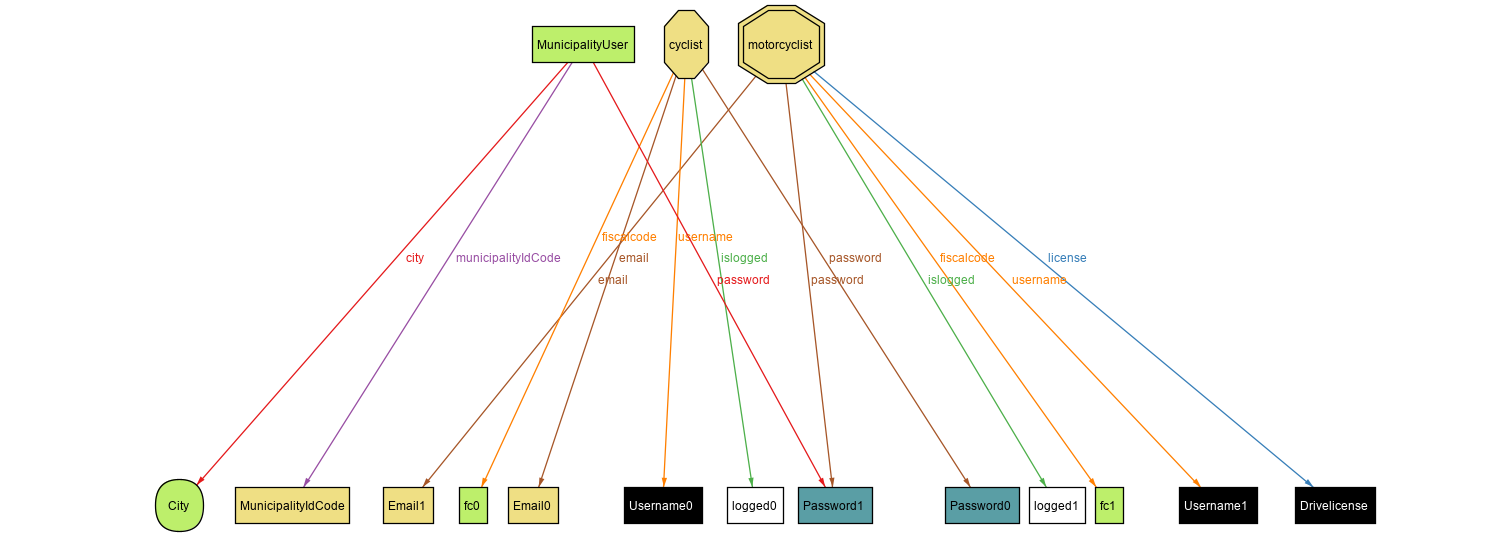
\includegraphics[scale=0.66, angle=90]{Alloy images/staticViewUsers.png}
	\centering
	\caption{Static view of the users of the application}
\end{figure}
\FloatBarrier
As you can see in the image above that each private user has a unique fiscal code, a unique email and a unique user-name. The other aspect can be equal to the ones of other users (they can be shared between different private users in the alloy model). The aspects that can be non unique are: the password and finally the state of the logging.\\
The Municipality users have a password, a code which identifies uniquely the municipality and finally the city of which the municipality refers. In this case the municipality users can have the same id code and the same city. This is the case in which they belong to the same municipality.
\paragraph{World 2:}
In this world we will show a view of how the violation reports are managed. We will show how the S2B will manage some aspect of the system which are the following:
\begin{itemize}
	\item The reports of the violations.
	\item The concept of dangerousness of the streets in the system.
	\item The traceability of the streets on the system.
	\item The set of the most dangerous streets.
	\item The mining of the information given by the 		
	municipality and the one given by the reports.
\end{itemize}
\begin{figure}[h]
	\includegraphics[scale=0.67,angle=90]{Alloy images/staticViewViolations.png}
	\centering
	\caption{Static view of the violations of the application}
\end{figure}
\FloatBarrier
As you can see in the image above, a street can be considered dangerous or not. It depends on the number of reports. It is considered dangerous if and only if the number of reports is 10\% greater than the average number of violations per street reported by the users or 10\% greater than the average violation per street retrieved from the municipality DB. This is respected in the world above.\\
The streets which have the same name but they are different are distinguished expressing also the city of which they belongs.\\
The system mine also the information about accidents of the municipality in order to have better information about the safety.
\paragraph{World 3:}
In this world we will show a complete view of the system in its completeness. Every aspect of the two worlds above will be shown.

\begin{figure}[h]
	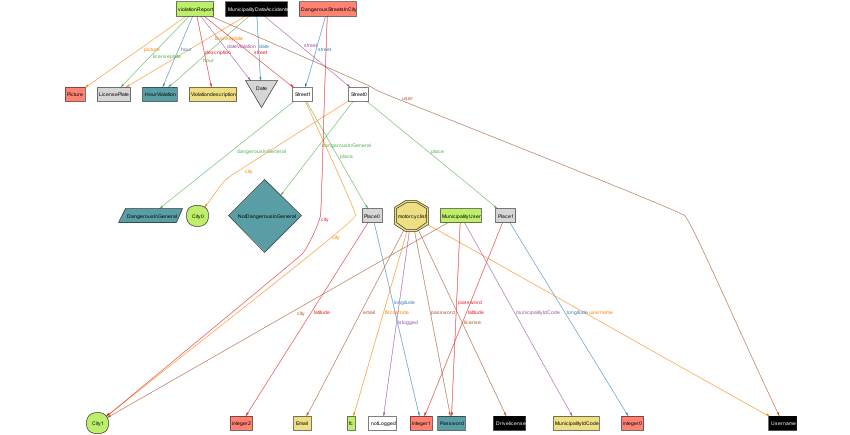
\includegraphics[scale=1.1,angle=90]{Alloy images/staticCompleteView.png}
	\centering
	\caption{Static complete view of the application}
\end{figure}
\FloatBarrier


\begin{figure}[h]
	\paragraph{Consistency:}
	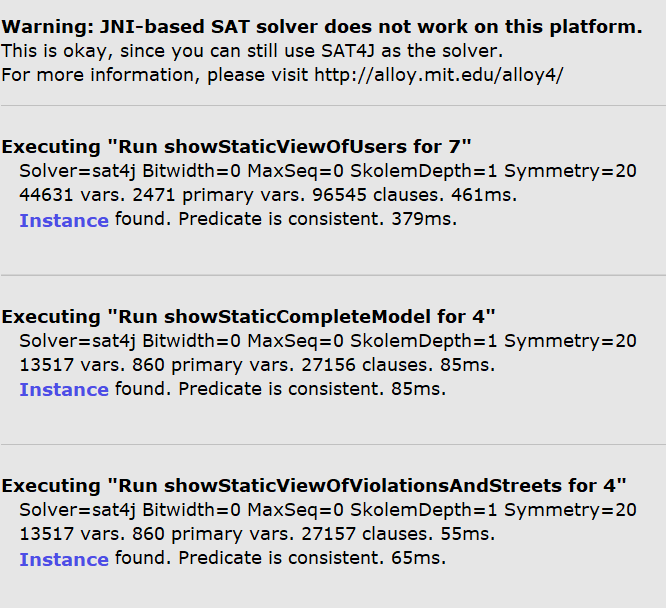
\includegraphics[scale=1.168]{Alloy images/Consistency of the model.png}
	\centering
	\caption{Consistency}
\end{figure}
\FloatBarrier
\newpage
\section{Effort}
\begin{longtable}{| p{12 cm} | p{2 cm} |} 
		\hline
		{\bf Task} & {\bf Hours}\\
		\hline
		 Git setup & 1 \\
		 Group work on chapter 1 & 3 \\
		 Writing in latex of sections 1.1 and 1.2 (purpose and scope) (already done in group) & 2 \\
		 Section 2.1 & 2,5 \\
		 State chart diagram & 1 \\
		 Section 2.2 (Product functions) & 2 \\
		 Half of section 2.3 (User characteristics) & 2 \\
		 Half of section 2.4 & 2 \\
		 Section 3.1 & 2\\
		 Use case diagrams & 3 \\
		 Mockups & 6\\
		 Scenarios & 3 \\
		 Alloy & 15\\
		 Chapter 4 review & 3\\
		 
		 Document Modification after the revision of the
		 tutor and discussion with the tutor (Group Work) & 10 \\
		\hline
		&  {\bf Total} \\
		\hline
		&  57.5 \\
		\hline
		\caption{Luca Massini's effort}
	\end{longtable}
	
	
	
	\begin{longtable}{| p{12 cm} | p{2 cm} |} 
		\hline
		{\bf Task} & {\bf Hours}\\
		\hline
		 Git setup & 1 \\
		 Group work on chapter 1 & 3 \\
		 Sections 1.3, 1.4, 1.5 & 1 \\
		 Section 1.6 & 1 \\
		 Section 2.1.1 (class diagrams) & 2\\ 
		 Half of section 2.3 (User characteristics) & 2 \\
		 Half of section 2.4 & 2 \\
		 Review of chapters 1 and 2 & 5 \\
		 Section 3.1 (Mockups insertion in latex and description) & 7\\
		 Use cases tables & 8 \\
		 Sequence diagrams & 8 \\
		 Section 3.2.5 & 3 \\
		 Sections 3.3, 3.4, 3.5 & 1.5 \\
		 Chapter 3 review & 2 \\
		 Document Modification after the revision of the
		 tutor and discussion with the tutor (Group Work) & 10 \\
		\hline
		&  {\bf Total} \\
		\hline
		&  56.5 \\
		\hline
		\caption{Daniele Nicolò's effort}
	\end{longtable}

\end{document}



